% Standalone TikZ figure: Domain Gap Visualization
% For Chapter 6: Domain Adaptation and Sim-to-Real Transfer
\documentclass[tikz,border=10pt]{standalone}
\usepackage{tikz}
\usepackage{amsmath}
\usetikzlibrary{arrows.meta, positioning, shapes.geometric, fit, backgrounds, calc, patterns, decorations.pathreplacing}

\begin{document}
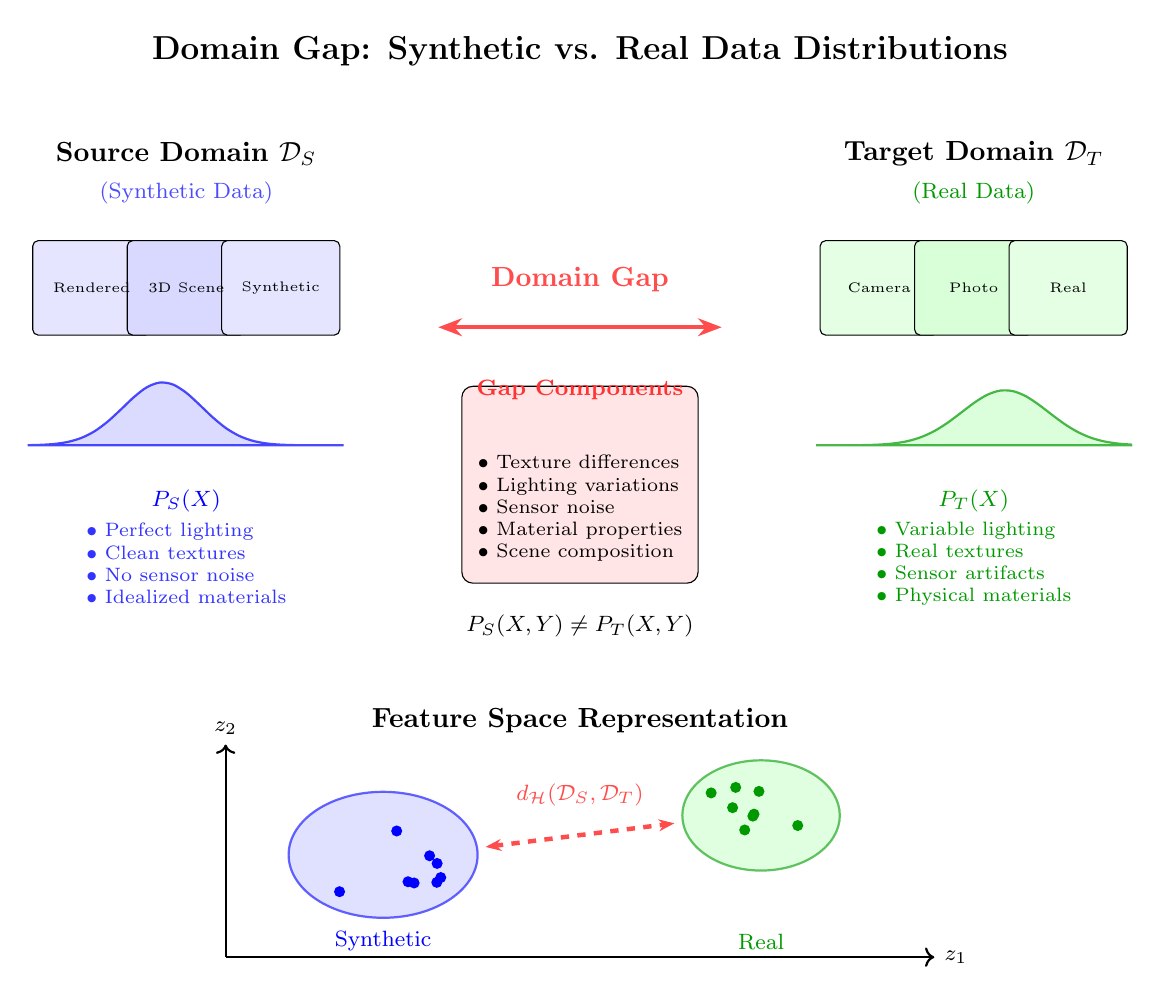
\begin{tikzpicture}[
    node distance=1.5cm,
    every node/.style={font=\small},
    arrow/.style={-{Stealth[length=2mm]}, thick},
    label/.style={font=\footnotesize}
]

% Title
\node[font=\bfseries\large] at (5, 4.5) {Domain Gap: Synthetic vs. Real Data Distributions};

% ============ SOURCE DOMAIN (SYNTHETIC) ============
\begin{scope}[shift={(0, 0)}]
    \node[font=\bfseries] at (0, 3.2) {Source Domain $\mathcal{D}_S$};
    \node[font=\footnotesize, text=blue!70] at (0, 2.7) {(Synthetic Data)};

    % Sample synthetic images (simplified representation)
    \node[draw, fill=blue!10, minimum width=1.5cm, minimum height=1.2cm, rounded corners=2pt] (syn1) at (-1.2, 1.5) {};
    \node[draw, fill=blue!15, minimum width=1.5cm, minimum height=1.2cm, rounded corners=2pt] (syn2) at (0, 1.5) {};
    \node[draw, fill=blue!10, minimum width=1.5cm, minimum height=1.2cm, rounded corners=2pt] (syn3) at (1.2, 1.5) {};

    % Simple icons inside boxes
    \node[font=\tiny] at (syn1) {Rendered};
    \node[font=\tiny] at (syn2) {3D Scene};
    \node[font=\tiny] at (syn3) {Synthetic};

    % Distribution curve
    \draw[thick, blue, fill=blue!20, opacity=0.7]
        plot[smooth, domain=-2:2] (\x, {0.8*exp(-(\x+0.3)^2/0.5) - 0.5})
        -- (2, -0.5) -- (-2, -0.5) -- cycle;
    \node[blue, font=\footnotesize] at (0, -1.2) {$P_S(X)$};

    % Characteristics
    \node[align=left, font=\scriptsize, text=blue!80] at (0, -2) {
        $\bullet$ Perfect lighting\\
        $\bullet$ Clean textures\\
        $\bullet$ No sensor noise\\
        $\bullet$ Idealized materials
    };
\end{scope}

% ============ GAP INDICATOR ============
\begin{scope}[shift={(5, 0)}]
    % Double-headed arrow showing gap
    \draw[ultra thick, red!70, {Stealth[length=3mm]}-{Stealth[length=3mm]}] (-1.8, 1) -- (1.8, 1);
    \node[font=\bfseries, red!70] at (0, 1.6) {Domain Gap};

    % Gap components
    \node[draw, rounded corners, fill=red!10, minimum width=3cm, minimum height=2.5cm] at (0, -1) {};
    \node[font=\bfseries\footnotesize, red!80] at (0, 0.2) {Gap Components};

    \node[align=left, font=\scriptsize] at (0, -1.3) {
        $\bullet$ Texture differences\\
        $\bullet$ Lighting variations\\
        $\bullet$ Sensor noise\\
        $\bullet$ Material properties\\
        $\bullet$ Scene composition
    };

    % Mathematical representation
    \node[font=\footnotesize] at (0, -2.8) {$P_S(X,Y) \neq P_T(X,Y)$};
\end{scope}

% ============ TARGET DOMAIN (REAL) ============
\begin{scope}[shift={(10, 0)}]
    \node[font=\bfseries] at (0, 3.2) {Target Domain $\mathcal{D}_T$};
    \node[font=\footnotesize, text=green!60!black] at (0, 2.7) {(Real Data)};

    % Sample real images (simplified representation)
    \node[draw, fill=green!10, minimum width=1.5cm, minimum height=1.2cm, rounded corners=2pt] (real1) at (-1.2, 1.5) {};
    \node[draw, fill=green!15, minimum width=1.5cm, minimum height=1.2cm, rounded corners=2pt] (real2) at (0, 1.5) {};
    \node[draw, fill=green!10, minimum width=1.5cm, minimum height=1.2cm, rounded corners=2pt] (real3) at (1.2, 1.5) {};

    % Simple icons inside boxes
    \node[font=\tiny] at (real1) {Camera};
    \node[font=\tiny] at (real2) {Photo};
    \node[font=\tiny] at (real3) {Real};

    % Distribution curve (shifted)
    \draw[thick, green!60!black, fill=green!20, opacity=0.7]
        plot[smooth, domain=-2:2] (\x, {0.7*exp(-(\x-0.4)^2/0.6) - 0.5})
        -- (2, -0.5) -- (-2, -0.5) -- cycle;
    \node[green!60!black, font=\footnotesize] at (0, -1.2) {$P_T(X)$};

    % Characteristics
    \node[align=left, font=\scriptsize, text=green!60!black] at (0, -2) {
        $\bullet$ Variable lighting\\
        $\bullet$ Real textures\\
        $\bullet$ Sensor artifacts\\
        $\bullet$ Physical materials
    };
\end{scope}

% ============ BOTTOM: FEATURE SPACE VIEW ============
\begin{scope}[shift={(5, -5.5)}]
    \node[font=\bfseries] at (0, 1.5) {Feature Space Representation};

    % Coordinate system
    \draw[->, thick] (-4.5, -1.5) -- (4.5, -1.5) node[right, font=\footnotesize] {$z_1$};
    \draw[->, thick] (-4.5, -1.5) -- (-4.5, 1.2) node[above, font=\footnotesize] {$z_2$};

    % Source domain cluster
    \draw[thick, blue, fill=blue!20, opacity=0.6] (-2.5, -0.2) ellipse (1.2cm and 0.8cm);
    \foreach \i in {1,...,8} {
        \pgfmathsetmacro{\px}{-2.5 + 0.8*rand}
        \pgfmathsetmacro{\py}{-0.2 + 0.5*rand}
        \fill[blue] (\px, \py) circle (2pt);
    }
    \node[blue, font=\footnotesize] at (-2.5, -1.3) {Synthetic};

    % Target domain cluster (shifted)
    \draw[thick, green!60!black, fill=green!20, opacity=0.6] (2.3, 0.3) ellipse (1.0cm and 0.7cm);
    \foreach \i in {1,...,8} {
        \pgfmathsetmacro{\px}{2.3 + 0.7*rand}
        \pgfmathsetmacro{\py}{0.3 + 0.4*rand}
        \fill[green!60!black] (\px, \py) circle (2pt);
    }
    \node[green!60!black, font=\footnotesize] at (2.3, -1.3) {Real};

    % Gap arrow
    \draw[ultra thick, red!70, dashed, {Stealth[length=2mm]}-{Stealth[length=2mm]}] (-1.2, -0.1) -- (1.2, 0.2);
    \node[red!70, font=\footnotesize, above] at (0, 0.3) {$d_{\mathcal{H}}(\mathcal{D}_S, \mathcal{D}_T)$};
\end{scope}

\end{tikzpicture}
\end{document}
